\section{Discussion} \label{discussion}
% Generel introduktion til at vi har trænet modeller og attLSTM var den bedste og bla bla ikke så stor forskel for høj redundancy
% swapped negatives og true negatives
During this thesis, multiple models have been trained to test different architectures' ability to predict TCR-pMHC interactions, where all neural network models outperformed a sequence similarity-based model. However, all models experienced a severe drop in performance as the redundancy was reduced. Here the LSTM with attention outperformed the other models and managed to retain some performance. The attLSTM achieved a performance of 0.88 across all peptides and up to 0.91 on certain individual peptides. The model focuses on areas containing the largest difference in sequences logos between positive and negative sequences. Attention may therefore explain why the model outperformed the normal LSTM, that is forced to propagate the signal through the entire sequence.

Experimenting with architectures is important when making machine learning models. However, equally important is ensuring the input data is of good quality and relevant for creating predictions. Using features that do not contribute information makes the model larger and more prone to overfit biases in the dataset. By training models and varying the number of features and sequences in the model, we showed that a small model containing a BLOSUM encoding of the peptide and CDR3s was significantly better than a model containing all features available from the dataset.

Lastly, peptide-specific models generally outperformed pan-specific models when a large number of observations were available for that peptide. in situations where training data was limited, the pan-specifc model and the pre-trained peptide-specific model regularly outperformed the peptide-specific model.

For further comparisons, it would be interesting to how the attLSTM model compared to the full NetTCR-2.0 model \cite{Montemurro2021NetTCR-2.0Data} or another LSTM based model ERGO \cite{Springer2020PredictionPairs}. The CNN baseline used in this thesis is a simplified model compared to NetTCR-2.0, as the full NetTCR-2.0 contains filters of multiple lengths (1, 3, 5, 7 and 9) as opposed to the simpler model used here with filters of length 3. The full NetTCR-2.0 obtains similar performance in their paper to what is achieved here. However, as the dataset has been modified during this thesis, the comparison is not completely valid, and a benchmarking on the same dataset would be required to compare performances accurately.

\subsection{Data biases}
The data used for this project have a heavy bias towards specific peptides. This lack of data for other peptides does limit the model's applicability to only a few peptides. A way to solve this issue is to develop tools and models that perform well in cases where few observations for specific peptides are available. Here the pan attLSTM model showed promise by being more resilient to having less training data than other models. Another solution is generating additional data for both the current and all-new peptides, which would bypass the problem by simply having more data available. 

By increasing the number of peptides in the data, there would be more peptides with higher similarity. It is reasonable to assume peptides with high similarity will bind similar TCRs. The model could have an easier time incorporating information from other peptides than currently, as the available peptides might be too dissimilar to provide information helpful in predicting other peptides. Increasing the amount of data will thereby make models better at generalizing and predicting less frequent peptides by leveraging information from other peptides.

The germline genes also contain large biases especially for positive TCRs (Figure \ref{fig:tcra_genes}-\ref{fig:tcrb_genes}). These biases can occur for different reasons. The experiments conducted to generate the data may introduce technical biases in the data if there is a preference toward TCRs with specific germlines due to the experimental design. The bias could also naturally occur in TCRs binding a specific peptide, meaning the data is representative of the general population of peptides binding that peptide. If this is the case and the model learns to separate the positive and negative TCRs, then the model has learned something general about TCR-pMHC interactions and not just an artefact in the dataset.

Therefore, checking if the observations with the common germlines originate from the same experiment or if multiple experiments find the same germlines to be overrepresented could give some insight into whether this is a technical bias in the data generation or a natural bias in TCRs binding these peptides.

% Har nævnt at der er bias i specielt GIL og derfor opnåes der mærkelige resultater
% Natural bias vs technical bias

% Comparison with NetTCR-2.0
\subsection{Introducing additional features to input}
Using only CDR3 and peptides gave the best results in the current dataset. CDR3 is the TCR loop closest to the peptide and contains the most sequence variation, but all CDR loops interact with the pMHC complex in some way. However, the information gained about TCR-pMHC binding is limited for CDR1 and CDR2 as they primarily interact with the MHC molecule \cite{Davis1988T-cellRecognition}.

The model currently only predicts TCR-pMHC binding for peptides binding the HLA-A02*01. Ideally, models should include predictions for peptides specific to other MHCs. In this setting, there may be a gain in introducing the MHC, CDR1 and CDR2, as they can contribute information specific to interactions between the MHC and TCRs. These types of information are probably not required for the current dataset, as all observations contain the same MHC, and the model does not need to understand these interactions to function.

In the thesis by Meitil, the energy features gave a performance increase in a leave peptide out setting \cite{Meitil2021UsingPrediction}. Here, we saw that all features gave the same performance as only using the sequence in a redundant setting and excluded the energy features for simplicity. The attLSTM has similar properties to the energy features in the thesis by Meitil, as it is superior when data becomes less redundant. The energy features may be able to boost performance further when the amount of data is limited compared to only using the sequence encoding and therefore be helpful on peptides with limited data. 

% Why is there a difference between maxpooling positions and attention (might be because of too many filters in the CNN only contributing noise and not taking the following hidden layers into account (low weights after)) (does the thresholding actually remove performance)

\subsection{Capturing multiple sequence motifs}
We saw the attention managed to capture one specific motif in the CNN and attLSTM model. In NetTCR-2.0, the model performance is boosted by having multiple filter lengths, which allows the model to capture multiple motifs. In CNNs, this is quite simple as the number of filters can be increased to capture different motifs from the ones already selected by max pooling. In the current form, attLSTM only captures one motif for each CDR3 and peptide. This was especially clear for the CDR3{\textalpha}, where it specifically found a QGN motif in TCRs positive towards GIL.

To extend the current implementation of attention and be able to capture multiple motifs in a sequence, the q (query) vector could be turned into a matrix (Figure \ref{fig:att_diag_discuss}). Here each row vector would be the high-level representation of a good motif same way a q is in the current implementation (Figure \ref{fig:attention_schema}). Doing this would increase the output from containing the weighted average according to one motif to have multiple weighted averages and allow the model to capture multiple types of motifs from the same sequence.

Increasing the number of motifs searched for may not give the desired increase in performance on the less frequent peptides in the current dataset. This is because the data is quite biased toward a specific GIL pattern, and there is no guarantee that the model learns motifs for other peptides. Instead, the model might learn other spurious details about GIL to increase performance on the most abundant peptide further. However, only searching for one motif is probably too simplistic, considering the level of variability between TCRs \cite{Sewell2012WhyCross-reactive}.
% limited to one type of good word/motif. More attentions might allow to capture what is important for the other peptides

\begin{figure}
    \centering
    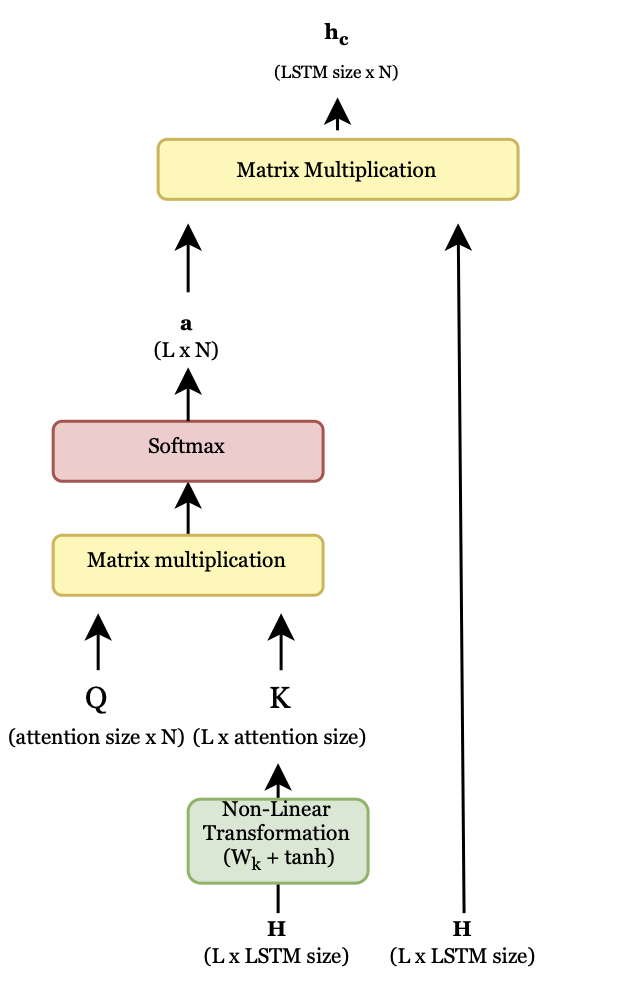
\includegraphics[scale=0.38]{figures/attention_diagram_discuss.png}
    \caption{Simple modification on the attention mechanism used in this project (Figure \ref{fig:attention_schema}). Q is now an N x attention size matrix capable of capturing N motifs instead of one.}
    \label{fig:att_diag_discuss}
\end{figure}

\subsection{Further exploring sequence embeddings}
CDR3-specific embeddings did not give the performance boost compared to a BLOSUM encoding. Here we trained the embeddings using a Word2Vec model generating per residue embeddings. Previous studies have also experimented with generating embeddings per 3-mer \cite{Asgari2015ContinuousGenomics, Yang2018LearnedLearning} and found these embeddings to capture physio-chemical properties of the sequences. The 3-mer embeddings used in these papers were created using the same method as here. These motif embeddings could either replace or supplement the per residue embeddings, which could prove superior to only the per residue embeddings used in this thesis.

Within NLP, transformers have gained much attention for their ability within language modelling \cite{Vaswani2017AttentionNeed}. The transformer has also led to the BERT model \cite{Devlin2019BERT:Understanding}, which is capable of creating word embeddings for the English language. The embeddings are learned in a self-supervised (unsupervised) manner and used for downstream applications such as text classification. BERT has also gained traction within protein language modelling with ESM \cite{doi:10.1073/pnas.2016239118} trained on 250 million evolutionary diverse sequences. Transformer based models are all based on the same idea of self-attention, where words/amino acids are predicted from their context. The models are significantly larger than the relatively small Word2Vec model. These more complex embeddings might be a better way to represent amino acids and could provide a performance boost to epitope prediction.

Recently TCR-BERT \cite{Wu2021TCR-BERT:Analyses} a CDR3{\textbeta} specific BERT model has been released for predicting TCR specificity. TCR-BERT uses an overall embedding for the CDR3{\textbeta} instead of per residue embeddings. The global CDR3{\textbeta} embeddings are used as input to a PCA-SVM classifier trained to predict a specific peptide. This approach differs from the one taken in this thesis, where we created per residue embeddings and used them to train a neural network classifier. So while a BERT model has been developed for TCR-pMHC prediction, it only utilizes the CDR3{\textbeta} and would probably benefit from incorporating CDR3{\textalpha} as seen in this thesis. Additionally, it would be interesting to see if the global embeddings of the sequences are better for predicting TCR-pMHC binding than training a neural network classifier using sequence embeddings generated from a TCR-specific BERT model.

\subsection{Pan specific vs peptide specific models}
We saw that pan-specific models generally rivalled the peptide-specific models' performance, especially when data became limited. As paired TCR sequencing is expensive, it is important that models work with small amounts of data. The number of TCRs required for a peptide to obtain meaningful performance needs to be reduced, as the number of potential epitopes is huge and obtaining 100-150 positive TCRs for each is unrealistic. Therefore, the pan-specific model is probably the best-suited model for this purpose. Another clear advantage of the pan-specific model is the convenience of only having one single model and being able to do specificity predictions using the model. Training peptide-specific models for the peptides available now is possible but will become infeasible as data for more peptides becomes available. Therefore, pan-specific models are preferred in the future due to the added stability and performance when the amount of data is limited.

The pre-training of peptide-specific models does rescue some of the issues when only a few observations are available for that peptide. However, the small gain in performance might not justify the increased number of models and losing the ability to make specificity predictions. It is unknown if pre-training a peptide-specific model on a pan-specific dataset even helps with specificity predictions. It would be nice to see whether this was the case, as that could prove the pre-training affects the model's ability to learn peptide specificity.

We saw all models drop in performance when there were fewer than 100-150 positive observations for the GIL peptide. This range was also mentioned by Montemurro et al. as the number of TCRs required to obtain meaningful performance \cite{Montemurro2021NetTCR-2.0Data}. It is unknown whether this hold for other peptides, as too few positives were available for these peptides to test it.


